\chapter{Användning av workshops för kompetensutveckling
  av Sebastian Callh}

\section{Introduktion}
\label{cha:seba-introduction}
När mjukvaruutveckling sker i grupp är det viktigt att gruppmedlemmarna innehar tillräcklig kompetens,
och det finns flertalet sätt att se till att så är fallet. Ett sätt att utbilda en grupp
är att hålla i en \textit{workshop}, där gruppen arbetar tillsammans för att lära sig relevant
teori och utföra en eller flera uppgifter för att få praktisk erfarenhet.

\subsection{Syfte}
\label{sec:seba-aim}
Syftet med den här rapporten är att redogöra för hur en workshop kan användas
för att hjälpa en grupp med skilda kompetenser att förbättra sin produktivitet i ett
mjukvaruutvecklingsprojekt, främst i aspekterna vilket innehåll och vilka verktyg som lämpar sig.

\subsection{Frågeställningar}
\label{sec:seba-research-questions}

\begin{enumerate}
\item Kan en workshop för en grupp där individerna har skilda förkunskaper höja deras effektivitet?

\item Hur bör man välja vilka ämnen som ska tas upp i en workshop?

\item Hur bra är PowerPoint för att förmedla kunskap inom mjukvaruutveckling på en workshop?

\item Hur bra är Live-kodning för att förmedla kunskap inom mjukvaruutveckling på en workshop? 
\end{enumerate}

\subsection{Avgränsningar}
\label{sec:seba-delimitations}
Studien baserades endast på kandidatarbetet som utfördes av
grupp två i kursen TDDD96 på Linköpings universitet våren 2017.

\section{Bakgrund}
När grupp två sattes samman för att utföra sitt kandidatarbete vårterminen 2017 hade gruppens
medlemmar mycket skilda kompetenser. För att gruppen skulle kunna bli produktiv 
så snabbt som möjligt var det viktigt att alla medlemmar fick tillräckligt med förkunskaper för
att kunna förstå och utföra deras uppdrag samt kommunicera med kund och varandra med ett
gemensamt vokabulär. Gruppens utvecklingsledare tog på sig uppdraget att tillgodose
kompetensbehovet och beslutade om att hålla en workshop med de verktyg som projektet
omfattade.

\section{Teori}
\label{cha:seba-theory}
I det här kapitlet förklaras centrala begrepp för studien.

\subsection{Workshop}
En workshop är en metod för att låta en grupp arbeta tillsammans för att åstadkomma ett gemensamt mål.
Vanligtvis bearbetas problem relaterade till ens arbetsplats eller yrke. \cite{facilitation_made_easy}
Den vaga definitionen gör att termen workshop dyker upp
inom många områden, men i den här rapportens kontext används en workshop 
för kompetensutveckling och kan betraktas som ett tillfälle för en grupp att ta
till sig ny teoretisk kunskap inom mjukvaruutveckling och tillämpa den praktiskt.
Det kan vara ett effektivt sätt att kompetensutbilda en grupp, så länge den utförs på ett bra sätt.
Viktiga aspekter som påverkar workshoppens framgång är vilket innehåll den har och vilket
medium som används för att presentera innehållet. 
\\ \\
Ett av de första momenten att betänka när man utför en workshop är vilket
ämne som den ska behandlas. \cite{facilitation_made_easy} För att finna ett bra ämne
bör frågan "Vilka behov av kompetensutveckling har gruppen?" besvaras \cite{facilitation_made_easy},
samtidigt som det är viktigt att ha i åtanke att en workshop ger mest värde om dess innehåll är
relevant för både ens organisation och för de som deltar i den.\cite{training_basics}
Deltagarnas intressen och åsikter om innehållet påverkar alltså hur lyckad en workshop blir.
\\ \\
Om man tar en hel grupps åsikter i åtanke när man planerar en workshop
kan den bli mycket bred i innehåll för att så många som möjligt ska uppskatta den.
En av de viktigaste aspekterna när man planerar en workshop är dock att
ha ett tydligt syfte \cite{facilitation_made_easy}, så ett mer fokuserat
upplägg är att föredra.

\subsection{Live-kodning}
Att live-koda innebär att skriva kod inför folk och är både ett underhållningsmedium och ett
pedagogiskt verktyg. Det har tidigare benämnts som det rekommenderade sättet att lära ut
mjukvaruutveckling. \cite{computer_science_teaching}

\section{Metod}
\label{cha:seba-method}
För att bestämma ett lämpligt ämne för en workshop utfördes en förstudie under vilken gruppen
observerades under arbete och diskussion för att försöka identifiera områden med potential
för kompetensutveckling. Gruppen fick även svara på ett frågeformulär med frågor relaterade
till de observationer som gjordes och deras kompetensnivåer.
\\ \\
Observationerna pågick en arbetsvecka varpå frågeformuläret distribuerades till gruppen.
Av observationerna kunde det konstateras att gruppens förståelse för hur automatiserad testning
gick till och dess fördelar var bristande. Detta bekräftades av svaren på frågeformuläret
som återges i \ref{tab:workshop_undersokning}.
\\ \\
Gruppen hade innan studien uttryckt ett missnöje med att
mycket tid spenderades i möten så ett internetfomulär valdes som metod för
att utföra studien. Internetformulär erbjuder flexibilitet och bekvämlighet i
när svarspersonerna svarar jämfört med metoder så som ansikte-mot-ansikte eller per telefon,
men har även nackdelar. Till exempel kan missförstånd lättare uppstå. \cite{questionnaire_design}
\\ \\
För att minimera mängden missförstånd följdes frågeformuläret upp i person under
ett möte med svarspersonerna då svaren diskuterades. På så sätt kunde det säkerställas att båda
parter tolkat svaren på samma sätt, och feltolkningar av frågor och svar kunde korrigeras.
Baserat på resultaten av undersökningen kunde det konstateras att en
workshop om Meteor och de ramverk och verktyg det bygger på skulle höja gruppens effektivitet,
varpå en litteraturstudie inom det påbörjades. Studien gick i huvudsak ut på att läsa dokumentation
på Internet om de olika teknikerna som använts i projektet.
\begin{table}[h!]
  \centering
  \caption{En tabell över områden lämpade för kompetensutveckling.}
  \def\arraystretch{1.5}
  \begin{adjustbox}{max width=\textwidth}
    \begin{tabularx}{\textwidth}{ | X | }
      \hline
      \textbf{Område} \\
      \hline
      Ramverket Meteor \\
      \hline
      JavaScript-exekveringsmiljön NodeJS \\
      \hline 
      NodeJS pakethanterare NPM \\
      \hline
      Meteor-paket \\
      \hline
      Enhetstester i Meteor med ramverket Chai \\
      \hline
    \end{tabularx}
  \end{adjustbox}
  \label{tab:workshop_kompetensutveckling}
\end{table}
\ \\
Efter några dagar avslutades litteraturstudien och områden som lämpade sig för kompetensutveckling
sammanfattades. Sammanfattningen återges i tabell \ref{tab:workshop_kompetensutveckling}.
För att hålla en fokuserad workshop bestämdes först ett scenario som deltagarna skulle få arbeta med.
Deras uppgift var att bygga ett system till regeringen för låtsaslandet \textit{Donaldknuthia}
enligt en mindre kravspecifikation som de fick tilldelade. Kravspecifikationen återfinnes i
 \ref{sec:workshop_kravspec_architecture}.
\ \\
Workshoppen delades upp i en teoretisk del och en praktisk del, och schemalades under två timmar.
Den teoretiska delen utgjordes av en presentation där materialet i tabell
\ref{tab:workshop_kompetensutveckling} bearbetades.
I undersökningen av vilka medium som lämpar sig bäst till att förmedla kunskap i en workshop
fokuserades det främst på PowerPoint och live-kodning som båda två visades på en projektor.
PowerPoint valdes för familjaritet från presentatören och för att anpassa mediet till
målgruppen då alla i gruppen var vana vid att det användes,
och live-kodning valdes eftersom det har visats ge positiv respons och underlätta
förståelse hos personer som har kunskap om programmering \cite{live_coding_for_all}.
Vid de tillfällen frågor dök upp som ej kunde besvaras med förberett material
improviserades kodexempel som visades på projektorn.
\\ \\
Svårighetsgraden som eftersträvades på workshoppen var låg. Eftersom deltagarna hade olika
kompetensnivåer gjordes en kompromiss där svårighetsgraden lades så pass låg att alla skulle kunna
följa med, men tempot höjdes någorlunda vid de enklare teoridelarna för att ge mer
tid åt svårare koncept.
\\ \\
Under den praktiska delen delades gruppen upp i par och uppmanades att implementera systemet de fått
beskrivet för sig. Frågor besvarades under tiden men deltagarna uppmuntrades att arbeta självständigt.
\\ \\
Efter workshoppen fick deltagarna fylla i ett frågeformulär där de olika
medierna utvärderades tillsammans med workshoppen upplevda relevans och kunskapsnivå.
Se \ref{tab:workshop_efter_formular} för frågeformuläret. Efter att den återstående
utvecklingsperioden i projektet passerat distribuerades ytterligare ett frågeformulär
för att ta reda på om produktiviteten förbättrats, vilka moment som faktiskt varit
användbara och vilka som saknades på workshoppen.

\section{Resultat}
\label{cha:seba-results}
Utifrån förstudien kunde det konstateras att det är viktigt att innehållet i en workshop bidrar
med värde till både ens organisation och deltagarna, samt att dess innehåll är fokuserat kring ett
centralt koncept. Man bör således försöka hitta innehåll kring samma koncept som är relevant
både för individen och för företaget när man planerar en workshop.
\\ \\
Svaren på utvärderingen efter workshoppen bekräftade att förstudien givit en korrekt bild av
gruppens kompetens då samtliga deltagare ansåg att innehållet var relevant för projektet.
Utvärderingen återges i \ref{tab:workshop_efter_formular}.
Utöver det fick användningen av PowerPoint 22 av 35 möjliga poäng och live-kodning 31 av 35
möjliga poäng där högre är bättre, vilket stödjer uttalandet om att live-kodning är ett bra
pedagogiskt verktyg för mjukvaruutveckling. Detta trots att vissa deltagare ansåg att personen
som höll i den gick för fort framåt. Det framgick även av utvärderingen att innehållet i
PowerPoint-presentationen inte upplevdes tillräckligt, vilket fick det att se tafatt ut.
\begin{figure}[ht!]
\centering
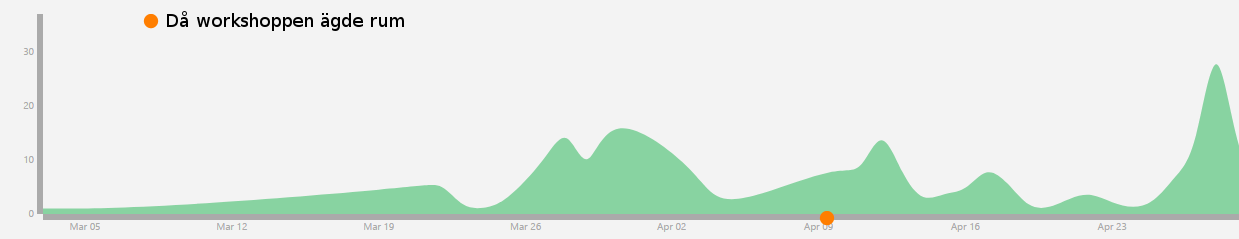
\includegraphics[width=\textwidth]{gitlab-graf}
\caption{En funktionskurva över mängden kodändringar i
  gruppens versionshanteringssystem med workshoppen utmärkt. \label{img:gitlab-graf}}
\end{figure}
\\ \\
Av den slutgiltiga utvärderingen som gjordes efter utvecklingsperioden kunde det konstateras
att 85,7\% av gruppen ansåg att workshoppen höjt deras effektivitet. Utvärderingen återges i
 \ref{tab:workshop_formular_efter_utveckling}. Det reflekterades också i
antal Trello-kort avklarade per dag som höjts från 0,45 till 0,6. I figur \ref{img:gitlab-graf}
ses dock gruppens kodändringar innan och efter workshoppen, där det inte går att se
märkbar skillnad.

\section{Diskussion}
\label{cha:seba-discussion}
I det här kapitlet diskuteras resultat och metod utifrån ett kritiskt synsätt.

\subsection{Resultat}
\label{sec:seba-discussion-results}
Resultaten av undersökningen av PowerPoint och live-kodning bör betraktas som subjektiva
eftersom de påverkas mycket av hur workshopledaren presterade.
Skulle personen till exempel tycka om att stå inför folk och ämnet hen presenterar ger det
en positiv påverkan av workshoppens resultat. 
\\ \\
14,3\% svarade att deras effektivitet ej förbättrats som följd
av workshoppen och att de gärna haft fler praktiska uppgifter.
Troligtvis beror det på att workshoppen var för enkel för dem,
vilket var förväntat eftersom den planerades med en svårighetsgrad
som skulle matcha den lägsta i gruppen.
\\ \\
Om den kvantitativa mätdata som fanns att tillgå betraktas så ser 
det ut som att workshoppen bidragit till förbättrad produktivitet.
Antal Trello-kort per dag ökade, men inte med stor
marginal, och produktivitet i projekt kan mycket väl
öka närmre deadlines av sig själv. Det var alltså svårt att säkert mäta någon förbättring
direkt kopplad till workshoppen vilket bekräftades av mätningen på antal kodändringar 
i gruppens versionshanteringssystem där det inte går att utläsa något direkt mönster.

\subsection{Metod}
\label{sec:seba-discussion-method}
I och med att studien endast omfattade åtta individer så är de slutsatser som dragits
högst subjektiva. En markant större testgrupp skulle behövas för att kunna dra några
allmänna slutsatser. Av samma anledning är det svårt att med säkerhet kunna återskapa
studien, då det är mycket beroende av vilka individer som ingår i gruppen. Som nämns
i \ref{sec:seba-discussion-results} så påverkar vem som håller i en workshop även
dess mottagande, så några säkra slutsatser om innehållet kan inte dras.
\\ \\
Under undersökningen gjordes inga jämförelser med hur gruppen skulle lärt sig
utan en workshop, vilket hade givit mycket god insikt. Tyvärr
är det omöjligt att undersöka då gruppmedlemmarna redan lärt sig workshoppens
material och ej kan glömma det. Med en större testgrupp skulle den dock kunna
delats in i två delar där en deltog i en workshop och den andra inte gjorde det,
varpå deras olika lärdomar skulle kunna jämföras.
\subsection{Arbetet i ett större perspektiv}
\label{sec:seba-work-wider-context}
En workshop är som mycket annat ett verktyg, och är
som koncept helt oberoende av vilket ämne som tas upp.
Det är fullt möjligt att använda en workshop till att
till exempel främja rasistiska åsikter, men även för att lära
ut hur man ger hjärt-och-lung-räddning. Studien
bryter dock ingen ny mark och kommer inte påverka
området märkbart.

\section{Slutsatser}
\label{cha:seba-conclusion}
En workshop har visat sig kunna höja en grupps effektivitet, så länge
den utförs på ett bra sätt. För att hitta ett bra ämne bör det 
undersökas vad deltagarna anser relevant, då deras attityd mot
workshoppens ämne i stor utsträckning påverkar hur väl de kommer lära sig.
Det är också viktigt att hålla en fokuserad workshop med ett centralt koncept
i kontrast till att ha en som tar upp många koncept väldigt ytligt.
\\ \\
Vad gäller pedagogiska verktyg är både live-kodning och PowerPoint användbara.
Live-kodning fungerar mycket bra för att förmedla programmeringskunskap, men
kräver att den som utför det är tydlig och inte går för fort framåt så att
åskådarna hinner med i resonemangen. PowerPoint är användbart
så länge det finns faktiskt material att visa upp, annars riskerar
det att se tafatt ut.